\documentclass[crop,tikz]{standalone}

\tikzset{>=latex}
\usetikzlibrary{decorations.markings}
\colorlet{green}{black!40!green}
\newcommand{\place}{\vec{r}}
\newcommand{\velocity}{\vec{v}}

\begin{document}
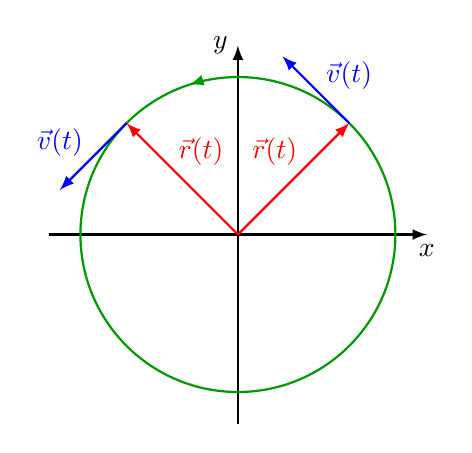
\begin{tikzpicture}[scale=2]
  \draw[->,thick] (-1.2,0) -- (1.2,0) node[below] {$x$};
  \draw[->,thick] (0,-1.2) -- (0,1.2) node[left] {$y$};
  \draw[
    decoration={markings, mark=at position 0.3 with {\arrow{>}}},
    postaction={decorate},
    green,
    thick
  ] (0,0) circle (1);
  % 1
  \draw[->,thick,red] (0,0) -- node[left,yshift=1em,xshift=0.5em] {$\place(t)$} (45:1);
  \draw[->,thick,blue] (45:1) -- node[right,yshift=0.5em]{$\velocity(t)$} +(135:0.6);
  % 2
  \draw[->,thick,red] (0,0) -- node[right,yshift=1em,xshift=-0.5em] {$\place(t)$} (135:1);
  \draw[->,thick,blue] (135:1) -- node[left,yshift=0.5em]{$\velocity(t)$} +(225:0.6);
\end{tikzpicture}
\end{document}
